%\documentclass{article}
%\documentclass[journal]{IEEEtran}
%\documentclass[letterpaper, twoside, openright]{report}
%\documentclass{ActaOulu}
%\documentclass[12pt, twoside]{memoir}

%%%---%%%---%%%---%%%---%%%---%%%---%%%---%%%---%%%---%%%---%%%---%%%---%%%

\documentclass[11pt,a4paper,oldfontcommands]{memoir}
\usepackage[utf8]{inputenc}
\usepackage[T1]{fontenc}
\usepackage{microtype}
\usepackage{times}

\usepackage[
breaklinks=true,colorlinks=true,
%linkcolor=blue,urlcolor=blue,citecolor=blue,% PDF VIEW
linkcolor=black,urlcolor=black,citecolor=black,% PRINT
bookmarks=true,bookmarksopenlevel=2]{hyperref}

\usepackage{geometry}
% PDF VIEW
% \geometry{total={210mm,297mm},
% left=25mm,right=25mm,%
% bindingoffset=0mm, top=25mm,bottom=25mm}
% PRINT
\geometry{total={210mm,297mm},
left=20mm,right=20mm,
bindingoffset=10mm, top=25mm,bottom=25mm}

\OnehalfSpacing
%\linespread{1.3}

%%% CHAPTER'S STYLE
\chapterstyle{bianchi}
%\chapterstyle{ger}
%\chapterstyle{madsen}
%\chapterstyle{ell}
%%% STYLE OF SECTIONS, SUBSECTIONS, AND SUBSUBSECTIONS
\setsecheadstyle{\Large\bfseries\sffamily\raggedright}
\setsubsecheadstyle{\large\bfseries\sffamily\raggedright}
\setsubsubsecheadstyle{\bfseries\sffamily\raggedright}

%%% STYLE OF PAGES NUMBERING
%\pagestyle{companion}\nouppercaseheads 
%\pagestyle{headings}
%\pagestyle{Ruled}
\pagestyle{plain}
\makepagestyle{plain}
\makeevenfoot{plain}{\thepage}{}{}
\makeoddfoot{plain}{}{}{\thepage}
\makeevenhead{plain}{}{}{}
\makeoddhead{plain}{}{}{}


\maxsecnumdepth{subsection} % chapters, sections, and subsections are numbered
\maxtocdepth{subsection} % chapters, sections, and subsections are in the Table of Contents


%%%---%%%---%%%---%%%---%%%---%%%---%%%---%%%---%%%---%%%---%%%---%%%---%%%


\usepackage{color}
\usepackage[usenames,dvipsnames]{xcolor}
\usepackage{graphicx}
\usepackage{rotating}
\usepackage{float}
\graphicspath{ {figures/ASUDS_block_diagram(s)_5-2-2015/} }
\usepackage{array}
\usepackage{authblk}
\usepackage{mathtools}
\usepackage{url}
\usepackage{hyperref}
\hypersetup{colorlinks=true, filecolor=blue, citecolor=red, linkcolor=blue, urlcolor=RoyalBlue, bookmarks=true}

\setcounter{tocdepth}{4}
\setcounter{secnumdepth}{4}

%%%---%%%---%%%---%%%---%%%---%%%---%%%---%%%---%%%---%%%---%%%---%%%---%%%


\begin{document}

\title{Ultrasonics Spectrometer Code Manual}
\author{Matthew Rothfuss\thanks{\href{mailto:mrengr@ksu.edu}{mrengr@ksu.edu}, \href{mailto:mrengr@phys.ksu.edu}{mrengr@phys.ksu.edu}}}
\affil{Department of Animal Science and Food Industry, Kansas State University}

\maketitle
\newpage
\tableofcontents

\chapter{LabView Basics}

\section{Introduction}

LabVIEW	(short	for	\textbf{Lab}oratory	\textbf{V}irtual	\textbf{I}nstrumentation	\textbf{E}ngineering	\textbf{W}orkbench) is a development environment for visual programming, developed by National Instruments (\href{http://www.ni.com/}{www.ni.com}). The code files (or program files) are identified by the \textbf{.vi} extension called \textbf{Virtual Instruments} or \textbf{VIs} for short. This graphical language is most commonly used for data acquisition, instrument control, signal processing (analysis), industrial automation, and more.

The next section will cover some basics of LabVIEW design and operation. For additional resources, the current (2013) LabVIEW Getting Started Manual is located \href{http://www.ni.com/pdf/manuals/373427j.pdf}{here}.

\subsection{Additional Resources}

\cite{gomez_alvarez-arenas_air-coupled_2003}

\chapter{Theory of Operation}

Define the background concepts of how/what this program is accomplishing.  Make refs to papers but don't do the math here (don't have time for that).  Just outline the basics of what we want to do, what goes into the system, what the system does (ref manuals and such for theory \& papers), and what the system outputs.

\chapter{Code Structure}

Theory of code operation goes here. ie case structure, state machine, 

\section{Main VI}

Define the outline of the Main VI (the main program) and hit on each part of it.  Don't spend time explaining the subvi's here since i'm doing that in the \textbf{Custom VI's} section. Make sure to to be thorough on all the code that is not included in the subvi section.

The main program \textbf{ASUDS\_v13.vi} is contained within a Project file called \textcolor{red}{(file name here)}. When the program is ran it will first load the auto generated system settings files (via the LC931C\_Read.vi [\ref{fig:LC931C_Read_main}] or DPR300\_Read.vi) [\ref{tab:jsr}]) from the last time the program ran. A set of default system settings files are included for first time use. Next the Oscilloscope and the JSR are both initialized via LC931C\_Int.vi and DPR300\_Int.vi [\ref{tab:osc}, \ref{tab:jsr}] with the loaded settings as-well-as set the front panel controls to the loaded settings. At the same time any leftover front panel controls are set to their default values and all block diagram cases are set to there initial positions.

Once the settings clusters have been set properly and

\section{Custom VI's}

List of custom VI's and a short description of what they do. In the next section we will take a deeper look into each of these subvi's.

These files load in most of the front panel controls, some are missing since more code has been added but the vi that saves the system settings has not been updated to include the new additions.

\subsection{Oscilloscope VIs}

\begin{table}[H]
	\centering
	\begin{tabular}{ m{2.5cm} | m{5cm} | m{5cm} }
		\hline
		\hline \multicolumn{3}{c}{Oscilloscope} \\ \hline \hline
		VI & File Name & Description \\ \hline
		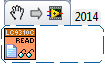
\includegraphics[scale=0.625]{LC931C_Read_main} & \hyperref[fig:LC9310C_Read_main]{LC9310C\_Read.vi} & Load Oscilloscope Setting from System Generated File \\ \hline
		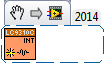
\includegraphics[scale=0.625]{LC931C_Int_main_02} & \hyperref[fig:LC9310C_Int_main_02]{LC9310C\_Int.vi} & Initialize Oscilloscope Settings \\ \hline
		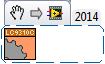
\includegraphics[scale=0.625]{LC931C_settings_main_01} & \hyperref[fig:LC9310C_settings_main_01]{LC9310C\_settings.vi} & Apply Settings to Oscilloscope \\ \hline
		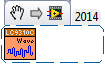
\includegraphics[scale=0.625]{LC931C_single-wave-output_main_01} & LC9310C\_single-wave-output.vi & Acquire Single Wave from Oscilloscope and Average \\ \hline
		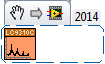
\includegraphics[scale=0.625]{LC931C_norm-pad-hilbert_main_01} & LC9310C\_norm-pad-hilbert.vi & Oscilloscope Tab Settings \\ \hline
		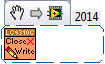
\includegraphics[scale=0.625]{LC931C-Config-Write-Close_main_01} & LC9310C-Config-Write-Close.vi & Write Oscilloscope settings to System File and close Oscilloscope resources \\ \hline
	\end{tabular}
	\caption{Oscilloscope Custom VIs}
	\label{tab:osc}
\end{table}

\subsubsection{LC9310C\_Read.vi}

\noindent\hrulefill

\begin{figure}[H]
	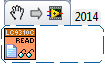
\includegraphics[scale=0.625]{LC931C_Read_main}
	\label{fig:LC9310C_Read_main}
\end{figure}

The LC931C\_Read.vi reads the LeCroy 9310C oscillosope settings from file and loads the values into a \textbf{LeCroy 9310C Settings} cluster. The settings folder (\textbf{System\_Settings}) is located in the root directory of the main VI. This VI requires the \href{http://sine.ni.com/nips/cds/view/p/lang/en/nid/209753}{MGI Library}. Figure (\ref{fig:LC931C_Read_blkdig}) is the block diagram.  It is setup as an error case structure. When an error is detected from the \textit{error (in)} input then the code in the green box does not execute.

The for loop steps through each list section of the ".ini" file. Each list section corresponds to one of the input cluster constants \textit{(LC930x\_TimeBase, LC930x\_Vertical\_Setup, LC930x\_Trigger\_Edge\_Setup, LC930x\_Read\_Wave)}. The \textbf{MGI Read Anything} VI needs to know the format of each section. This is accomplished by the cluster constants being converted into variants for the Read Anything variant input.  For more on the MGI VI's and how they operate, refer to their help manuals respectably. Once the \textbf{MGI Read Anything} VI has pulled out the relevant data, then the \textbf{variant to data} vi is used to reformat the output back to the cluster constant. The output for each cluster only executes when its section is read (hence the when integer counter =0. =1, =2, =3, then output data). 

\noindent\hrulefill \hyperref[tab:osc]{Back to Osc. Table \ref{tab:osc}}

\begin{sidewaysfigure}[p!]
	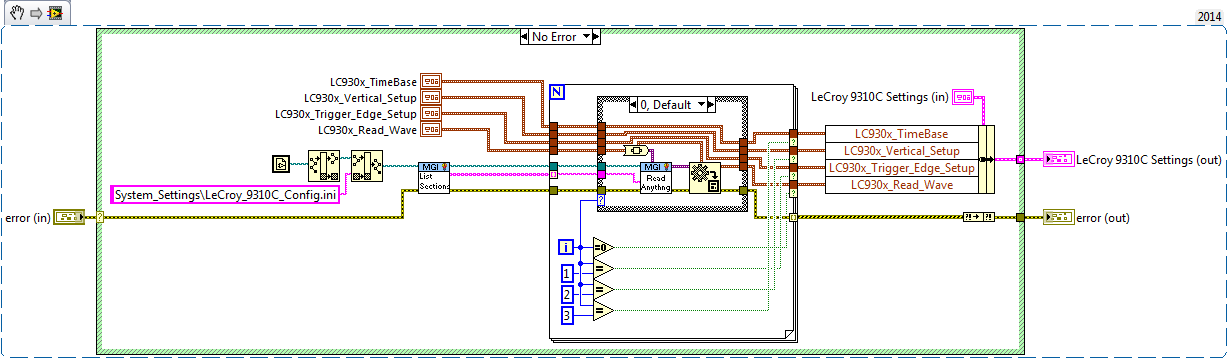
\includegraphics[width=\textheight,keepaspectratio]{LC931C_Read_blockdiagram}
	\caption{LC9310C\_Read.vi}
	\label{fig:LC9310C_Read_blkdig}
	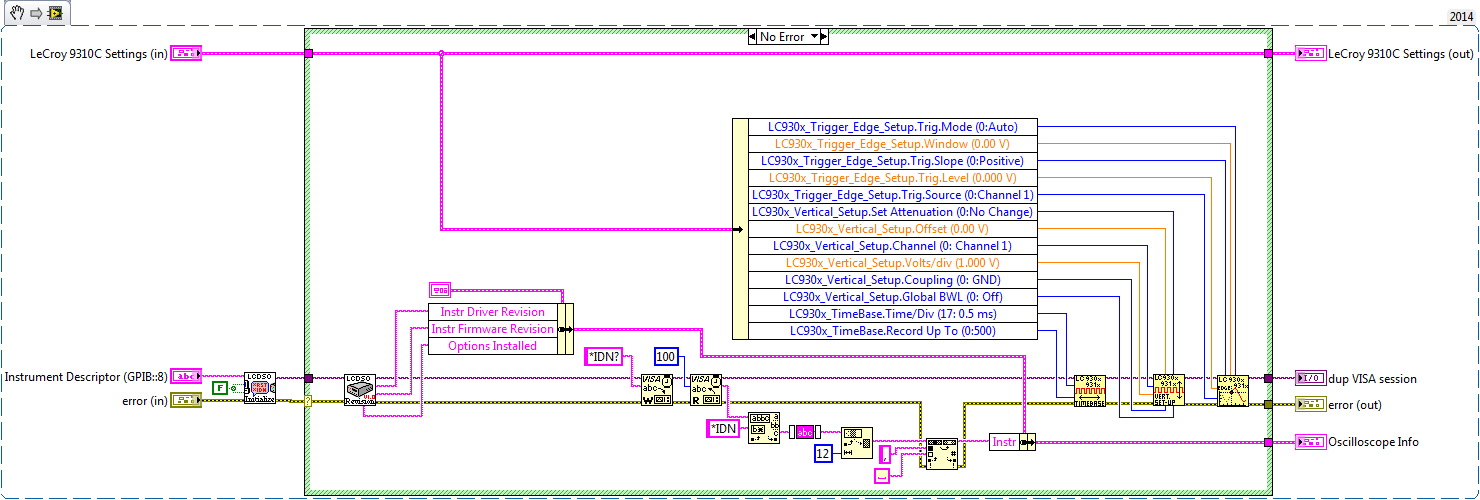
\includegraphics[width=\textheight,keepaspectratio]{LC931C_Int_blockdiagram}
	\caption{LC9310C\_Int.vi}
	\label{fig:LC9310C_Int_blkdig}
\end{sidewaysfigure}

\subsubsection{LC9310C\_Int.vi}

\noindent\hrulefill

\begin{figure}[H]
	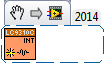
\includegraphics[scale=0.625]{LC931C_Int_main_02}
	\label{fig:LC9310C_Int_main_02}
\end{figure}

The LC931C\_Int.vi initializes the LeCroy 9310C Oscilloscope settings: \textit{trigger setup, vertical setup, and time setup (horizontal)}. This VI requires the \href{http://sine.ni.com/apps/utf8/niid_web_display.download_page?p_id_guid=E3B19B3E9608659CE034080020E74861}{LeCroy lc930x1x Library}. Figure (\ref{fig:LC9310C_Int_blkdig}) is the block diagram.  It is setup as an error case structure. When an error is detected from the \textit{error (in)} input then the code in the green box does not execute, instead the case not shown passes through the \textbf{LeCroy 9310C Settings} unchanged.

The \textbf{LCDSO Initialize} VI takes the GPIB location of the oscilloscope and creates a duped VISA session for the instrument. Next the \textbf{LCDSO Revision} reads the instruments Driver, Firmware, and Options Installed. All are put into a cluster called \textbf{Oscilloscope Info}, but first we write to the VISA session \textit{*IND?} an identification command. Next read the response with a count of 100 (the length of our expected response), this will give an identification string that is placed into the \textbf{Oscilloscope Info} cluster.

From the \textbf{LeCroy 9310C Settings} in cluster we set the \textbf{LC930x TimeBase}, \textbf{LC930x Vertical Setup}, and \textbf{LC930x Trigger} VIs. The cluster is unbundled and each setting is routed to it's respective input. Note the \textbf{LeCroy 9310C Settings} cluster is just passed through in this VI and not altered, because it is only pulling out data to setup other VIs.

\noindent\hrulefill \hyperref[tab:osc]{Back to Osc. Table \ref{tab:osc}}

\newpage

\subsubsection{LC9310C\_Settings.vi}

\noindent\hrulefill

\begin{figure}[H]
	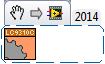
\includegraphics[scale=0.625]{LC931C_settings_main_01}
	\label{fig:LC9310C_settings_main_01}
\end{figure}

The LC931C\_Settings.vi applies changes to the \textit{trigger setup, vertical setup, and time setup (horizontal)} oscilloscope VIs. This VI requires the \href{http://sine.ni.com/apps/utf8/niid_web_display.download_page?p_id_guid=E3B19B3E9608659CE034080020E74861}{LeCroy lc930x1x Library}. Figure (\ref{fig:LC9310C_Int_blkdig}) is the block diagram. On the "error" case the \textbf{LeCroy 9310C Settings} cluster is passed through and so is the error cluster.

\noindent\hrulefill \hyperref[tab:osc]{Back to Osc. Table \ref{tab:osc}}

\begin{figure}[H]
	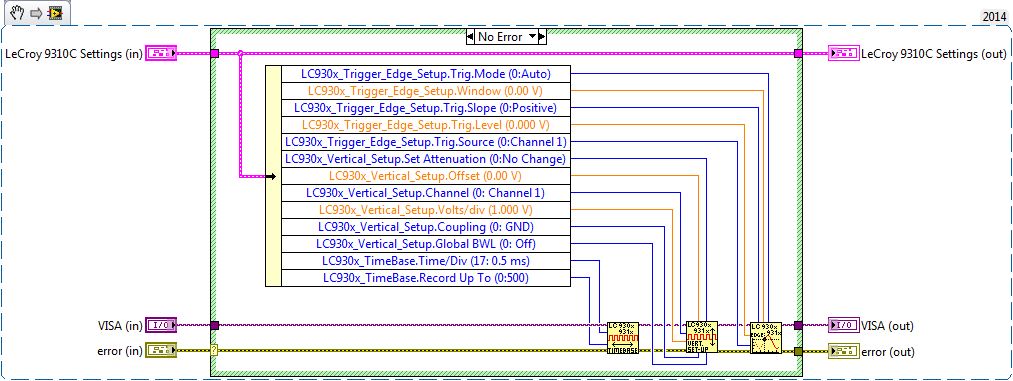
\includegraphics[width=\textwidth,keepaspectratio]{LC931C_settings_blockdiagram_01}
	\caption{LC9310C\_Settings.vi}
	\label{fig:LC9310C_settings_blkdig_01}
\end{figure}

\newpage

\begin{table}
	\centering
	\begin{tabular}{ m{2.5cm} | m{5cm} | m{5cm} }
		\hline
		\hline \multicolumn{3}{c}{JSR Pulser/Receiver} \\ \hline \hline
		VI & File Name & Description \\ \hline
		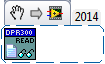
\includegraphics[scale=0.625]{DPR300_Read_main} & DPR300\_Read.vi & Load Pulser/Receiver Setting from System Generated File \\ \hline
		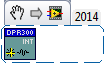
\includegraphics[scale=0.625]{DPR300_Int_main_02} & DPR300\_Int.vi & Initialize Pulser/Receiver Settings \\ \hline
		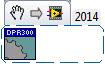
\includegraphics[scale=0.625]{DPR300_settings_main_01} & DPR300\_settings.vi & Apply Settings to Pulser/Receiver \\ \hline
		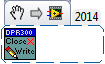
\includegraphics[scale=0.625]{DPR300-Config-Write-Close_main_01} & DPR300-Config-Write-Close.vi & Write Pulser/Receiver settings to System File and close Pulser/Receiver resources \\ \hline
	\end{tabular}
	\caption{JSR Pulser/Receiver Custom VI's}
	\label{tab:jsr}
\end{table}

\begin{table}
	\centering
	\begin{tabular}{ m{2.5cm} | m{5cm} | m{5cm} }
		\hline
		\hline \multicolumn{3}{c}{Ultrasonic Package} \\ \hline \hline
		VI & File Name & Description \\ \hline
		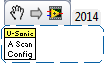
\includegraphics[scale=0.625]{USonic-A-Scan-Config-edit_main_01} & USonic-A-Scan-Config-edit.vi & Configure/Set Gates for Data Acquisition \\ \hline
		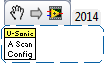
\includegraphics[scale=0.625]{USonic-A-Scan-Config-edit_main_01} & USonic-Gates-edit.vi & Pull Out Relevant Data from Gates for Data Acquisition \\ \hline
		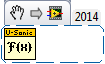
\includegraphics[scale=0.625]{USonic-FFT_main_01} & USonic-FFT.vi & Process Gate For Quick Analysis \\ \hline
	\end{tabular}
	\caption{Ultrasonic A-Scan Customized Package VI's}
	\label{tab:usonic}
\end{table}

\begin{table}
	\centering
	\begin{tabular}{ m {2.5cm} | m{5cm} | m{5cm} }
		\hline
		\hline \multicolumn{3}{c}{Math} \\ \hline \hline
		VI & File Name & Description \\ \hline
		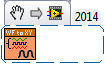
\includegraphics[scale=0.625]{Waveform-to-XY-Array_main_01} & Waveform-to-XY-Array.vi & Convert Waveform to XY-Array \\ \hline
		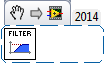
\includegraphics[scale=0.625]{Filter_signal_main_01} & Filter\_signal.vi & Filter Wave Signal for Oscilloscope Tab (does not affect Data Acquisition) \\ \hline
		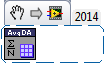
\includegraphics[scale=0.625]{Average-Dynamic-Array_main_01} & Average-Dynamic-Array.vi & Take the Average of N elements in a Dynamic Array \\ \hline
		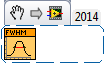
\includegraphics[scale=0.625]{FWHM-Poly_main_01} & FWHM-Poly.vi & Compute the Full Width Half Max (FWHM) of either a Waveform, XY-Graph, or Waveform cluster \\ \hline
		\hline
	\end{tabular}
	\caption{Custom Math VI's}
	\label{tab:math}
\end{table}

\begin{table}
	\centering
	\begin{tabular}{ m {2.5cm} | m{5cm} | m{5cm} }
		\hline
		\hline \multicolumn{3}{c}{Miscellaneous} \\ \hline \hline
		VI & File Name & Description \\ \hline
		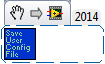
\includegraphics[scale=0.625]{Save-User-Config-File_main_01} & Save-User-Config-File.vi & Save all front panel controls to a user.ini settings file \\ \hline		
		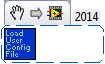
\includegraphics[scale=0.625]{Load-User-Config-File_main_01} & Load-User-Config-File.vi & Load the user.ini settings file \\ \hline
		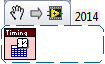
\includegraphics[scale=0.625]{Time-Data_main_01} & Time-Data.vi & Load and Save Data Timing table \\ \hline
		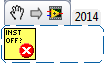
\includegraphics[scale=0.625]{Instrument-error-handler_main_01} & Instrument-error-handler.vi & Pop-up error message for loss of Instrument signal\\ \hline
		\hline
	\end{tabular}
	\caption{Miscellaneous Custom VI's}
	\label{tab:misc}
\end{table}

\section{Operation}



\bibliography{ultrasound-ref-01}
\bibliographystyle{unsrt}

\end{document}
